\chapter{Implementation of Evolution Scenarios}
\section{Docker}
 	As shown in figure \ref*{Deploym_CoCoME} the docker Container contains five different Glassfish servers. In particular they are called \textit{WEB}, \textit{ENTERPRISE}, \textit{STORE}, \textit{REGISTRY} and \textit{ADAPTER} and correspond to the given by the CoCoME deplyoment setup. By default, Glassfish provides a Derby DB that is connected to the server Adapter using Java Database Conectivity (JDBS) interface.\\
 	\begin{figure}[h]
 		\centering
 		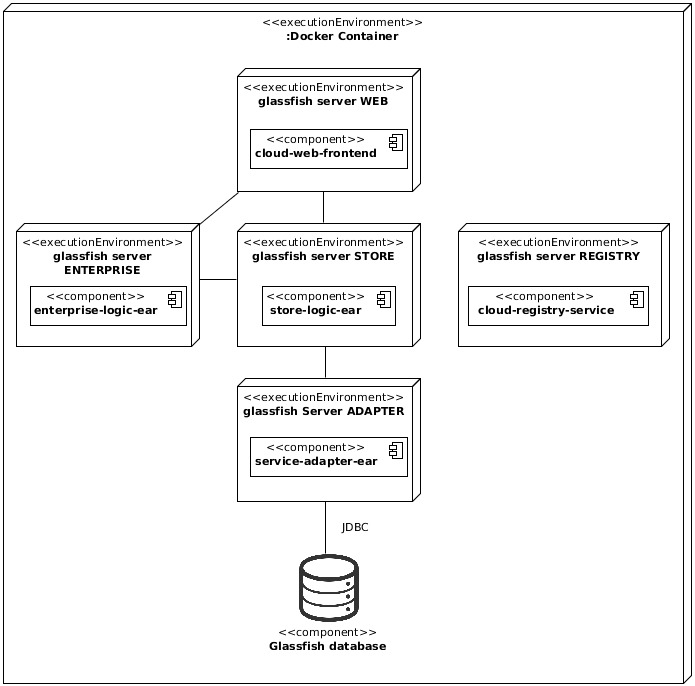
\includegraphics[width = 0.8\textwidth]{img/docker_Container_Deployment.png}
 		\caption{Deployment diagram CoCoME}
 		\label{Deploym_CoCoME}
 	\end{figure}
 	
 	CoCoME is deployed inside the docker container on the same way it is usually deployed. This means the maven generated archive files \textit{cloud-web-frontend},\textit{enterprise-logic-ear},\textit{store-logic-ear}\textit{cloud-registry-sevice} and \textit{service-adapter-ear} are deployed to the servers with the following assignment:
 	\begin{figure}[H]
 		\centering
 		\begin{tabular}{p{0.25\textwidth}|p{0.01\textwidth}p{0.25\textwidth}}
 			Server && Deployment file \\
 			\hline
 			WEB && cloud-web-frontend  \\
 			ENTERPRISE && enterprise-logic-ear  \\
 			STORE && store-logic-ear  \\
 			REGISTRY && cloud-registry-service  \\
 			ADAPTER && service-adapter-ear \\	
 		\end{tabular}
 		\caption{Assignment of archive files to Servers}
 		\label{table_assignment}
 	\end{figure}
 	\ref{table_assignment} demonstrates the assignment between the archive files and the servers as it is implemented and also recommended by the CoCoME deployment guide. This information is also represented in Fig. 2. As mentioned earlier, there are two versions of this Docker project. Both deploy the CoCoME main program with this assignment.\\ \\
 	
 	In addition, the fast version can be extends by the pickup shop\footnote{\url{https://github.com/cocome-community-case-study/cocome-cloud-jee-web-shop}}. This pickup-shop runs inside a separate container which is shown in figure \ref{Deploym_Pickup}.  
 	\begin{figure}[h]
 		\centering
 		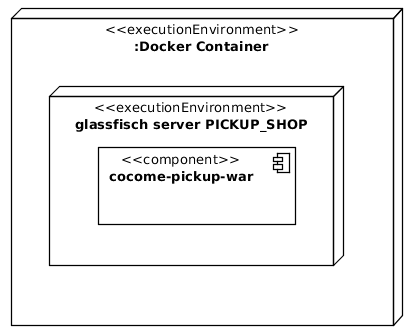
\includegraphics[width = 0.4\textwidth]{img/docker_Container_PickUP.png}
 		\caption{Deployment diagram CoCoME Pickup Shop}
 		\label{Deploym_Pickup}
 	\end{figure}
 	As shown in figure \ref*{Deploym_Pickup}, this container provides only one Glassfish server.
 	\begin{figure}[H]
 		\centering
 		\begin{tabular}{p{0.25\textwidth}|p{0.01\textwidth}p{0.25\textwidth}}
 			Server && Deployment file \\
 			\hline
 			PICKUP\_SHOP && cocome-pickup-war \\	
 		\end{tabular}
 		\caption{Assignment archive files to Servers}
 		\label{table_assignment_pickup}
 	\end{figure}
 	To control the start of both containers, precisely the CoCoME and the Pick Up Shop, another specific file is needed: the Docker Compose file. It ensures that the CoCoME Container is active, before the pickup-shop container is starting. This is necessary as the Pickup Shop requires a running instance of CoCoME to register itself.\\
 	Also CoCoME runs without the pickup-shop, the pickup-shop does not work without an running instance of CoCoME.\\
 	Both containers need to communicate with each other. By default, docker prohibits any outgoing and ingoing communication from an in a container. This is solved by opening specific ports through which the communication is possible. Which ports the containers can use is specified in the Docker Compose file as well.
 \section{Mobile App}\label{AppImplementation}